%%%%%%%%%%%%%%%%%%%%%%%%%%%%%%%%%%%%%%%%%%
%%%%%%%%%%%%%                 %%%%%%%%%%%%
%%%%%%%%%%%%%    EXERCISE 1   %%%%%%%%%%%%
%%%%%%%%%%%%%                 %%%%%%%%%%%%
%%%%%%%%%%%%%%%%%%%%%%%%%%%%%%%%%%%%%%%%%%
\begin{exercise}[]{Suppose the information content of a packet is the bit pattern 1110 0110 1001
    1101 and an even parity scheme is being used. What would the value of the field containing
    the parity bits be for the case of a two-dimensional parity scheme? Your answer should be
    such that a minimumlength checksum field is used. (15 points)}
  \begin{solution}
    The minimum length checksum is obtained when the row number and the column number are the same. The parity bits value are listed as follows (in the last column and last row).
  \end{solution}
  \begin{verbatim}
    1110 1
    0110 0
    1001 0
    1101 1

    1100 0
  \end{verbatim}
  \label{ex1}
\end{exercise}



%%%%%%%%%%%%%%%%%%%%%%%%%%%%%%%%%%%%%%%%%%
%%%%%%%%%%%%%                 %%%%%%%%%%%%
%%%%%%%%%%%%%    EXERCISE 2   %%%%%%%%%%%%
%%%%%%%%%%%%%                 %%%%%%%%%%%%
%%%%%%%%%%%%%%%%%%%%%%%%%%%%%%%%%%%%%%%%%%
\begin{exercise}[]{Consider the 5-bit generator, G=10011, and suppose that D has the value
    1010101010. What is the value of R? (10 points)}
  \begin{solution}
  \par{~}
  0100, because $1010101010\ 0000 = 10011 \times 1011011100 + 100$
  \end{solution}
  \label{ex2}
\end{exercise}


%%%%%%%%%%%%%%%%%%%%%%%%%%%%%%%%%%%%%%%%%%
%%%%%%%%%%%%%                 %%%%%%%%%%%%
%%%%%%%%%%%%%    EXERCISE 3   %%%%%%%%%%%%
%%%%%%%%%%%%%                 %%%%%%%%%%%%
%%%%%%%%%%%%%%%%%%%%%%%%%%%%%%%%%%%%%%%%%%
\begin{exercise}[]{Problem 3 Consider the previous problem 2, but suppose that D has the value (15 points)
    \begin{enumerate}
        \item 1001010101. (5 points)
        \item 0101101010. (5 points)
        \item 1010100000. (5 points)
    \end{enumerate} }
  \begin{solution}
  \par{~}
  \begin{enumerate}
    \item 0000, because $1001010101 \ 0000= 10011 \times 1000110000$
    \item 1111, because $0101101010 \ 0000= 10011 \times 0101010101 + 1111$
    \item 1001, because $1010100000 \ 0000= 10011 \times 1011010111 + 1001$
  \end{enumerate}
  \end{solution}
  \label{ex3}
\end{exercise}

\newpage

%%%%%%%%%%%%%%%%%%%%%%%%%%%%%%%%%%%%%%%%%%
%%%%%%%%%%%%%                 %%%%%%%%%%%%
%%%%%%%%%%%%%    EXERCISE 4   %%%%%%%%%%%%
%%%%%%%%%%%%%                 %%%%%%%%%%%%
%%%%%%%%%%%%%%%%%%%%%%%%%%%%%%%%%%%%%%%%%%
\begin{exercise}[]{4 Consider three LANs interconnected by two routers, as shown in Figure 1 (20 points)
    \begin{enumerate}
        \item Assign IP addresses to all of the interfaces. For Subnet 1 use addresses of the form
        192.168.1.xxx; for Subnet 2 uses addresses of the form 192.168.2.xxx; and for Subnet
        3 use addresses of the form 192.168.3.xxx. (5 points)
        \item Assign MAC addresses to all of the adapters. (5 points)
        \item Consider sending an IP datagram from Host E to Host B. Suppose all of the ARP
        tables are up to date. Enumerate all the steps, as done for the single-router example
        in Section 6.4.1 . (5 points)
        \item Repeat part 3, now assuming that the ARP table in the sending host is empty (and
        the other tables are up to date). (5 points)
    \end{enumerate}
    \begin{figure}[hb]
      \begin{center}
      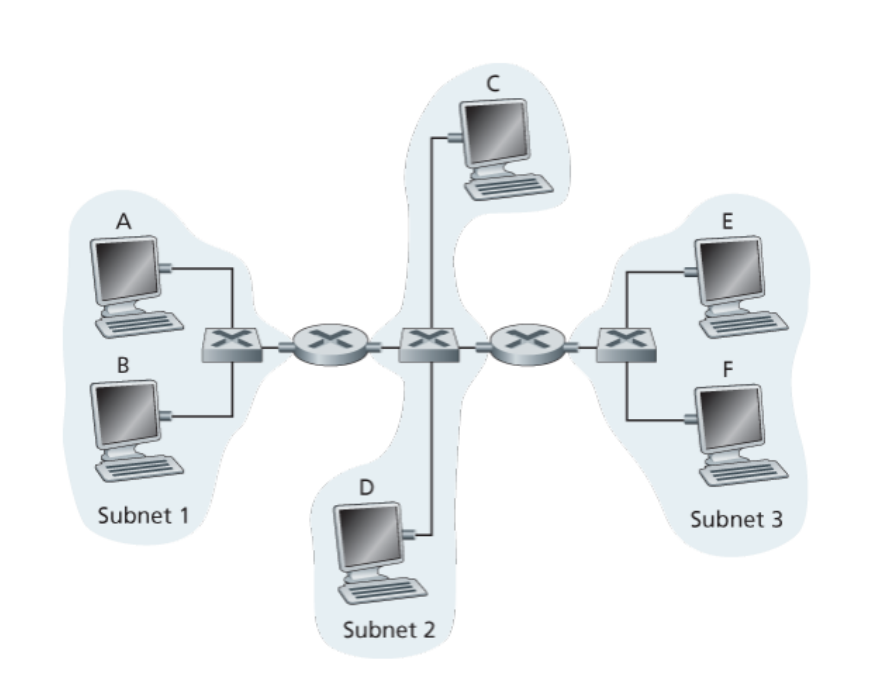
\includegraphics[width=8cm]{img/ass5/ex4}
      \caption{Three subnets, interconnected by routers}
      \label{fig:ex4}
      \end{center}
    \end{figure}
    }
  \begin{solution}
  \par{~}
  \begin{enumerate}
    \item See figure \ref{fig:ex4-ans}
    
    \begin{figure}[hb]
      \begin{center}
      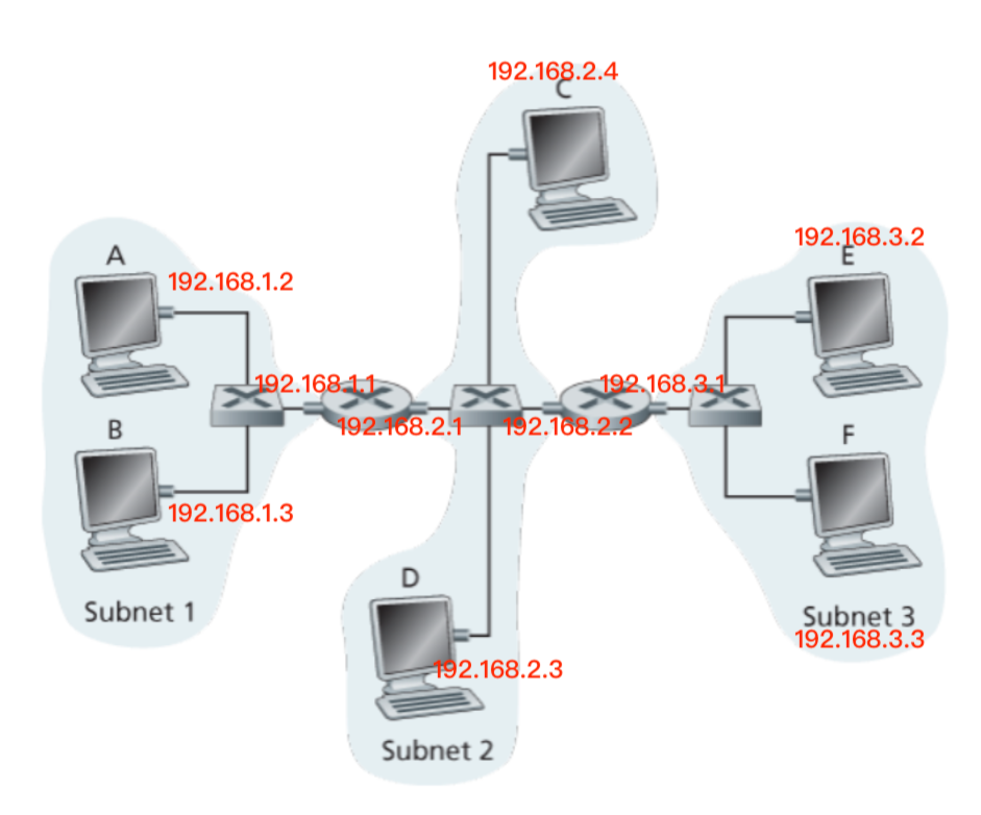
\includegraphics[width=8cm]{img/ass5/ex4-ans}
      \caption{Answer to Exercise \ref{ex4}}
      \label{fig:ex4-ans}
      \end{center}
    \end{figure}

    \item The MAC address should be assigned by the Internet administrating organizations. Each adapter in the Figure will have a unique MAC address like \texttt{90:9c:4a:c6:da:b7}.
    \item First, the sender E creates IP datagram with IP source E, destination B. Then E creates link-layer frame with the right router's MAC address as destination address, frame contains E-to-B IP datagram. Then, the frame sent from E to the right router frame is received, datagram is removed and passed up to IP. The right router will forward the datagram with IP source E, destination B and create link-layer frame with left router's MAC address as destination address, frame contains E-to-B IP datagram. Finally, the host B will receive the frame from the left router, passing it up to IP. The datagram is obtained.
    \item E will first use the ARP protocol to broadcast an ARP query packet, containing B's IP address and set destination MAC address as FF-FF-FF-FF-FF-FF. Then all nodes on LAN will receive ARP query. As for the router, since it knows the IP address, it will reply to E with its (router's) MAC address, so that the steps described in part 3 can resume.
  \end{enumerate}

  \end{solution}
  \label{ex4}
\end{exercise}


%%%%%%%%%%%%%%%%%%%%%%%%%%%%%%%%%%%%%%%%%%
%%%%%%%%%%%%%                 %%%%%%%%%%%%
%%%%%%%%%%%%%    EXERCISE 5   %%%%%%%%%%%%
%%%%%%%%%%%%%                 %%%%%%%%%%%%
%%%%%%%%%%%%%%%%%%%%%%%%%%%%%%%%%%%%%%%%%%
\begin{exercise}[]{ Suppose nodes A and B are on the same 10 Mbps broadcast channel, and the
    propagation delay between the two nodes is 325 bit times. Suppose CSMA/CD and Ethernet
    packets are used for this broadcast channel. Suppose node A begins transmitting a frame
    and, before it finishes, node B begins transmitting a frame. Can A finish transmitting before
    it detects that B has transmitted? Why or why not? If the answer is yes, then A incorrectly
    believes that its frame was successfully transmitted without a collision. Hint: Suppose at
    time t=0 bits, A begins transmitting a frame. In the worst case, A transmits a minimumsized frame of 512+64 bit times. So A would finish transmitting the frame at t=512+64 bit
    times. Thus, the answer is no, if B’s signal reaches A before bit time t=512+64 bits. In the
    worst case, when does B’s signal reach A? (20 points)}
  \begin{solution}
  \par{~} A can finish transmitting before it detects that B has transmitted. Assume A begins transmitting a frame at $0$. It will finish its transmission at $512+64$ bit times. B will receive the beginning of the frame at $325$ bit times. So before $325$, B is able to send out its frames. If B chooses to send its frame at time $251 ~ 324$, then the frame will arrive at A at a time later than $512 + 64$ bit times (after A has transmittted). Therefore, it is possible that A finish transmitting before it detects that B has transmitted.
  \end{solution}
  \label{ex5}
\end{exercise}



%%%%%%%%%%%%%%%%%%%%%%%%%%%%%%%%%%%%%%%%%%
%%%%%%%%%%%%%                 %%%%%%%%%%%%
%%%%%%%%%%%%%    EXERCISE 6   %%%%%%%%%%%%
%%%%%%%%%%%%%                 %%%%%%%%%%%%
%%%%%%%%%%%%%%%%%%%%%%%%%%%%%%%%%%%%%%%%%%
\begin{exercise}[]{Let’s consider the operation of a learning switch in the context of a network
    in which 6 nodes labeled A through F are star connected into an Ethernet switch. Suppose
    that (i) B sends a frame to E, (ii) E replies with a frame to B, (iii) A sends a frame to B, (iv)
    B replies with a frame to A. The switch table is initially empty. Show the state of the switch
    table before and after each of these events. For each of these events, identify the link(s) on
    which the transmitted frame will be forwarded, and briefly justify your answers. (20 points)}
  \begin{solution}
  \par{~}
  \begin{enumerate}
    \item When B sends a frame to E, the frame in transmission will be flooded to all links except the arriving interface in the network. After transmission, the switch will record the entry of B interface.
    \item When E sends a frame to B, the frame in transmission will be sent only to B interface since the entry has been learnt in the previous step. After transmission, the switch will have the entries of B and E interfaces.
    \item When A sends a frame to B, the frame in transmission will be sent only to B interface since the entry has been learnt in the first step. After transmission, the switch will have the entries of A, B and E interfaces.
    \item When B sends a frame to A, the frame in transmission will be sent only to A interface since the entry has been learnt in the previous step. After transmission, the switch will have the entries of A, B and E interfaces.
  \end{enumerate}
  \end{solution}
  \label{ex6}
\end{exercise}